\section{Linear Regression for Univariate Data}

The Basis Function takes the form,

\begin{equation*}
    \phi{(\mathbf{x})} = {\mathbf{x}^j} \tag{ $0 \leq j \leq Degree$}
\end{equation*}

\subsection{Results of change in regularisation parameter and degree of fit for training data =10}


Generally at lower degrees, the function does not well fit as can be observed from the plots [\ref{fig:1}]. For Degree 6 the function seems to fit well. On the contrary, for degree $9$, it overfits in the case of no regularisation constant. This can be explained by the less number of samples used in the training set and the degree being high. Once the regularisation constant is increased, it fits well till a certain point.

\newpage
\begin{figure}[!ht]
    \centering
    \begin{subfigure}[t]{0.25\textwidth}
        \centering
        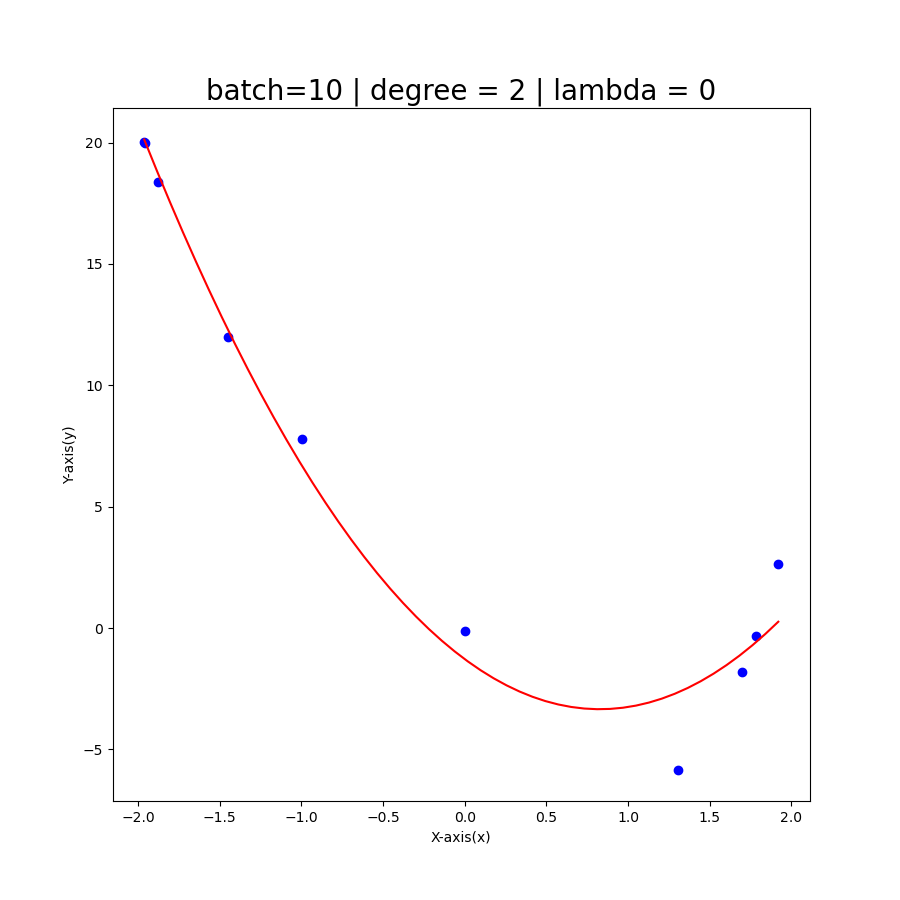
\includegraphics[height=1.5in]{Task 1 Images/Batch 10/Figure_1.png}
    \end{subfigure}%
    ~ 
    \begin{subfigure}[t]{0.25\textwidth}
        \centering
        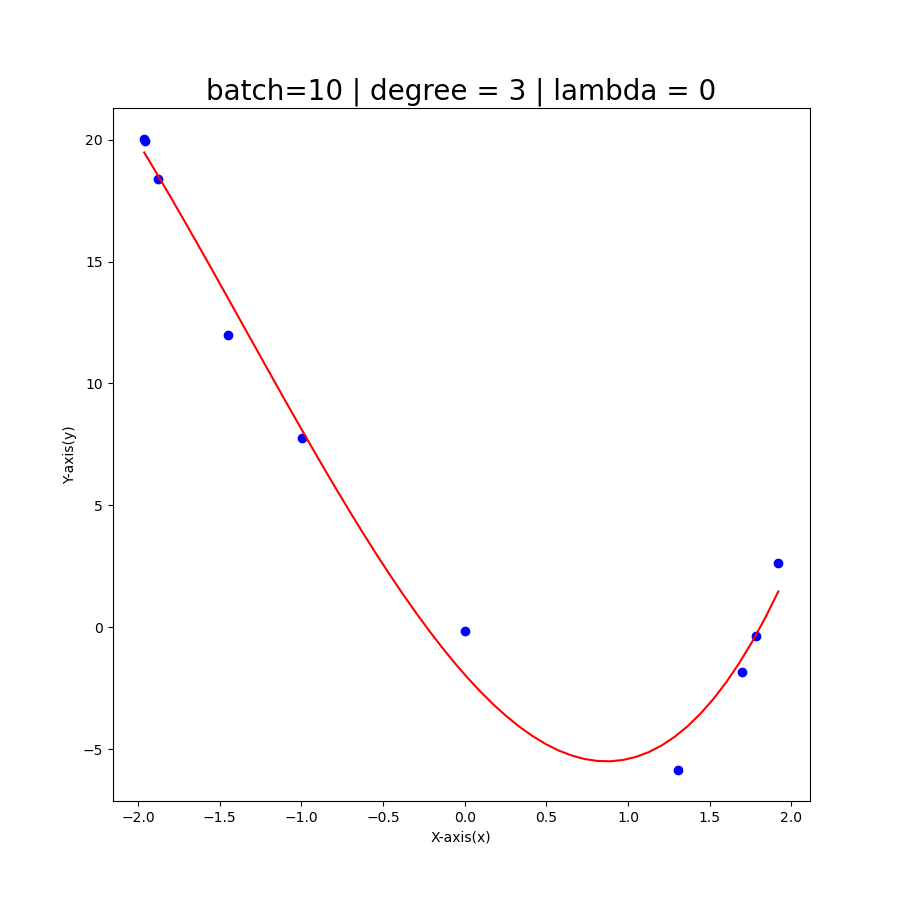
\includegraphics[height=1.5in]{Task 1 Images/Batch 10/Figure_2.png}
    \end{subfigure}%
    ~
    \begin{subfigure}[t]{0.25\textwidth}
        \centering
        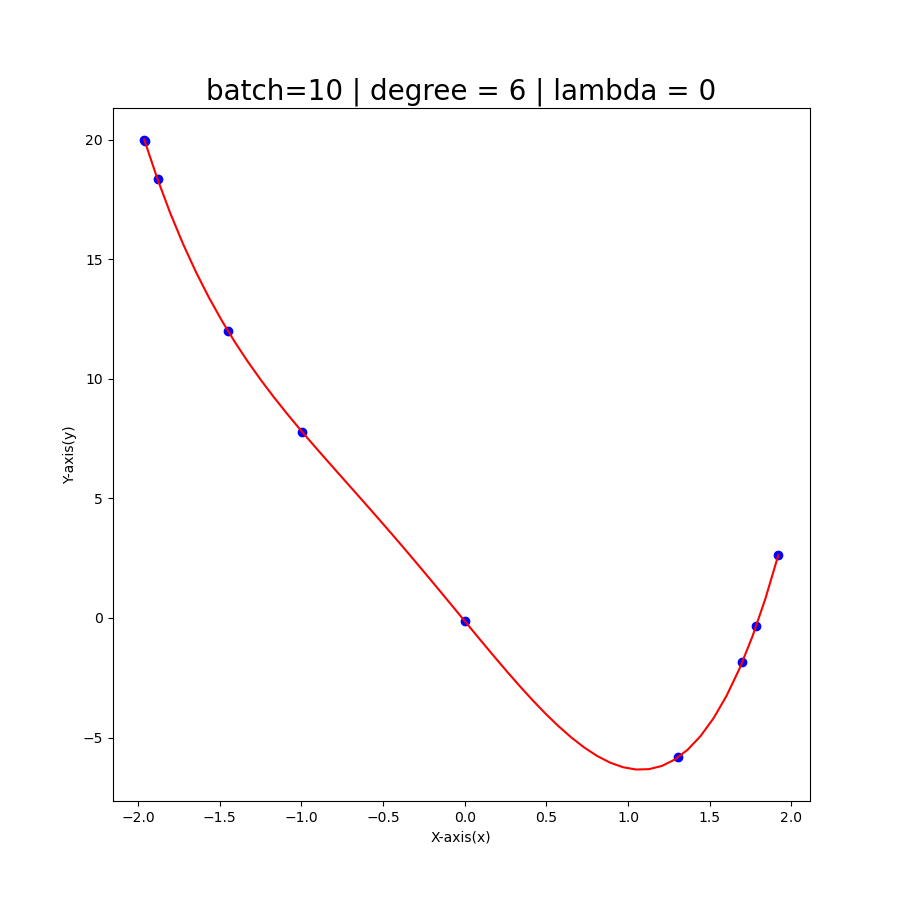
\includegraphics[height=1.5in]{Task 1 Images/Batch 10/Figure_3.png}
    \end{subfigure}%
    ~ 
    \begin{subfigure}[t]{0.25\textwidth}
        \centering
        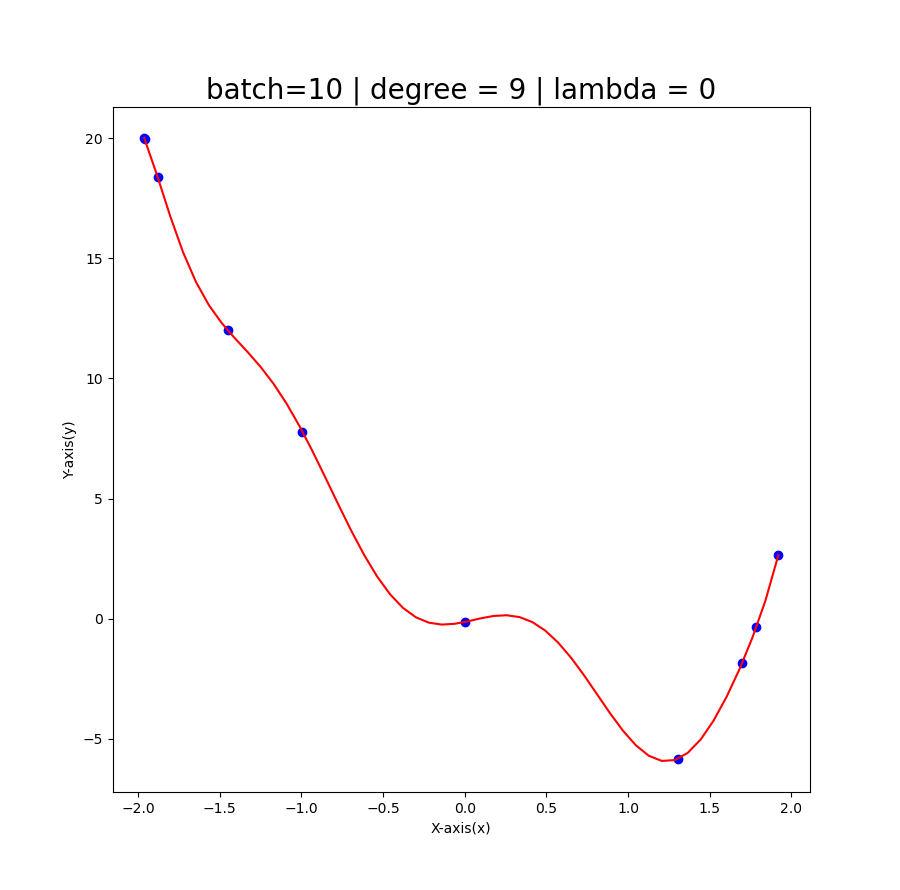
\includegraphics[height=1.5in]{Task 1 Images/Batch 10/Figure_4.png}
    \end{subfigure}%
    \caption{Plots of Polynomials having various orders of degree for a fixed regularisation parameter $\lambda = 0$ using batch size=10}
    \label{fig:1}
\end{figure}


{\rowcolors{3}{green!40!yellow!10}{green!0!yellow!30}
\begin{table}[!ht]
\begin{tabular}{ |p{1.5cm}|p{3cm}|p{3cm}| p{3cm}|  }
\hline
\multicolumn{4}{|c|}{$\mathbf{E}_{rms}$ values for different degrees } \\
\hline
\rowcolor{lightgray} \textbf{Degree} & $\mathbf{E}_{rms-train}$ & $\mathbf{E}_{rms-test}$ & $\mathbf{E}_{rms-valid}$ \\
2   &   1.38  &  1.83   &  2.00   \\   
\hline
 3   &  0.99 &  1.74  &  1.39   \\   
 \hline
 6   &   0.01   &   0.24   &   0.10         \\
 \hline
 9   &   5.4e-4   &    0.19        &     0.42     \\
 \hline
\end{tabular}
\caption{Error comparisons for varying degrees of $\phi(\mathbf{x}) $ for Dataset 1 using batch size=10}
\label{table:1}
\end{table}
}


Since degree 9 is overfit, we experiment with different regularisation parameter lambda the of quadratic regularisation term to see how it affects the fit. For lambda=0.001 and 0.01, the validation Erms decreases than what was before and from 0.1 it increases again. For higher values of lambda the fit is not proper as can be seen from the figures below[\ref{fig:2}].

\newpage
\begin{figure}[!ht]
    \centering
    \begin{subfigure}[ht]{0.5\textwidth}
        \centering
        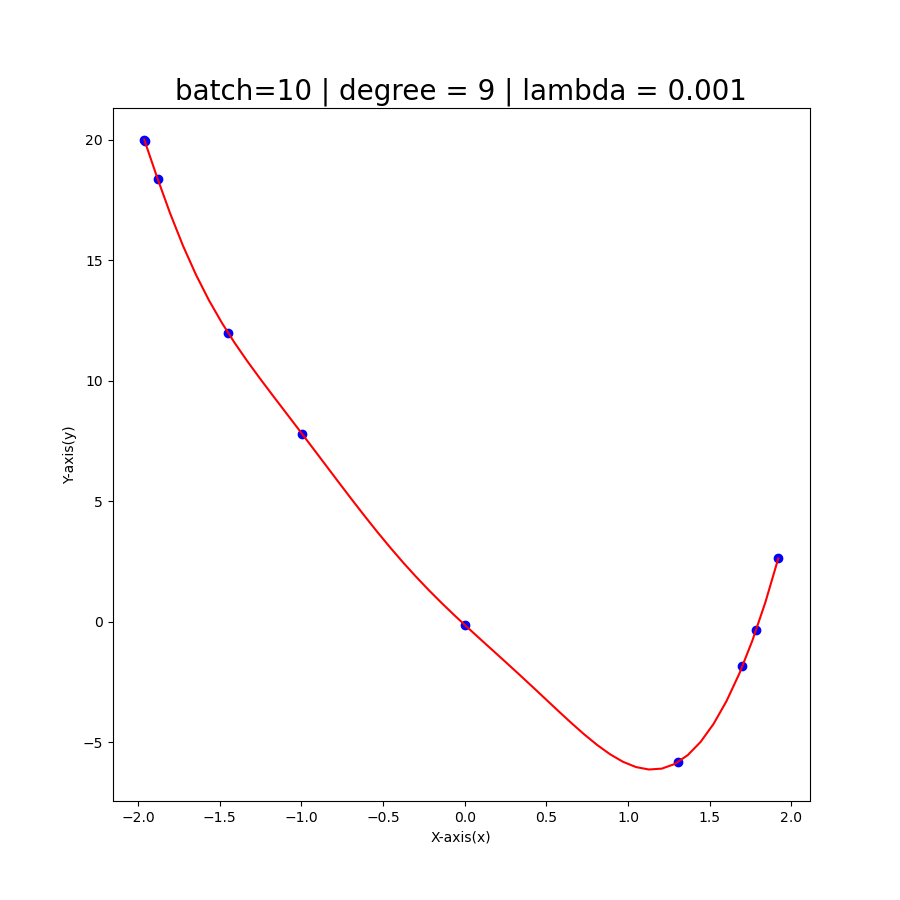
\includegraphics[height=2in]{Task 1 Images/Batch 10/Figure_5.png}
    \end{subfigure}%
    ~ 
    \begin{subfigure}[ht]{0.5\textwidth}
        \centering
        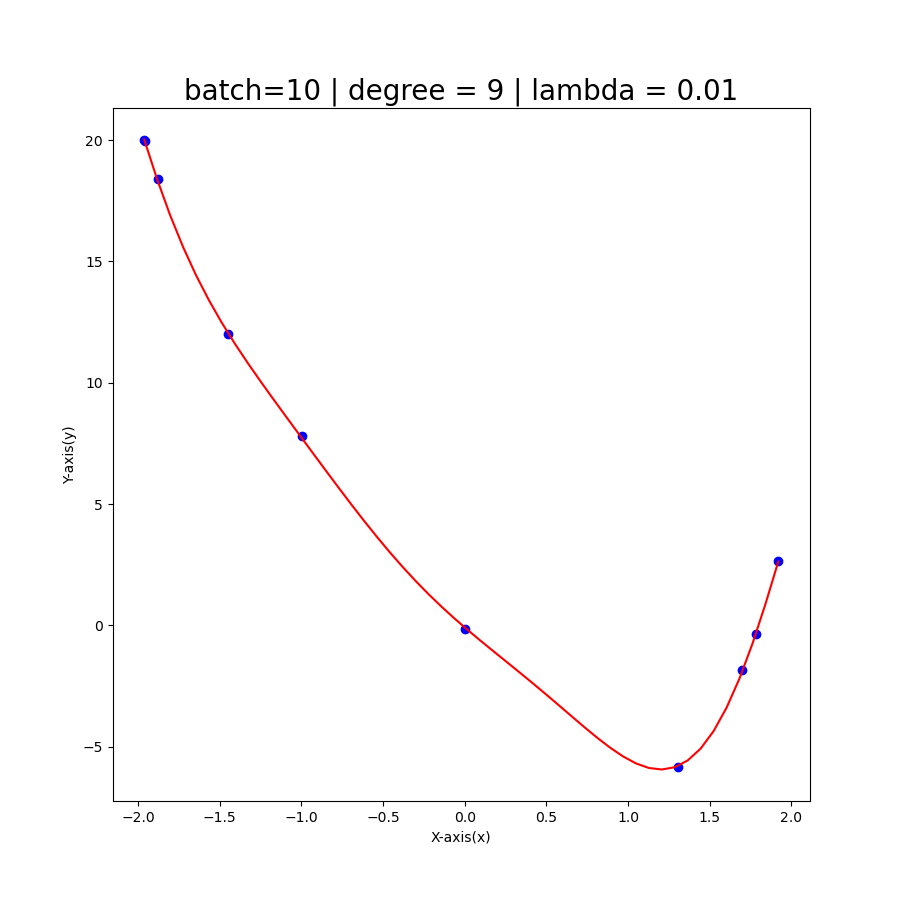
\includegraphics[height=2in]{Task 1 Images/Batch 10/Figure_6.png}
    \end{subfigure}%
    ~
    
    \begin{subfigure}[ht]{0.5\textwidth}
        \centering
        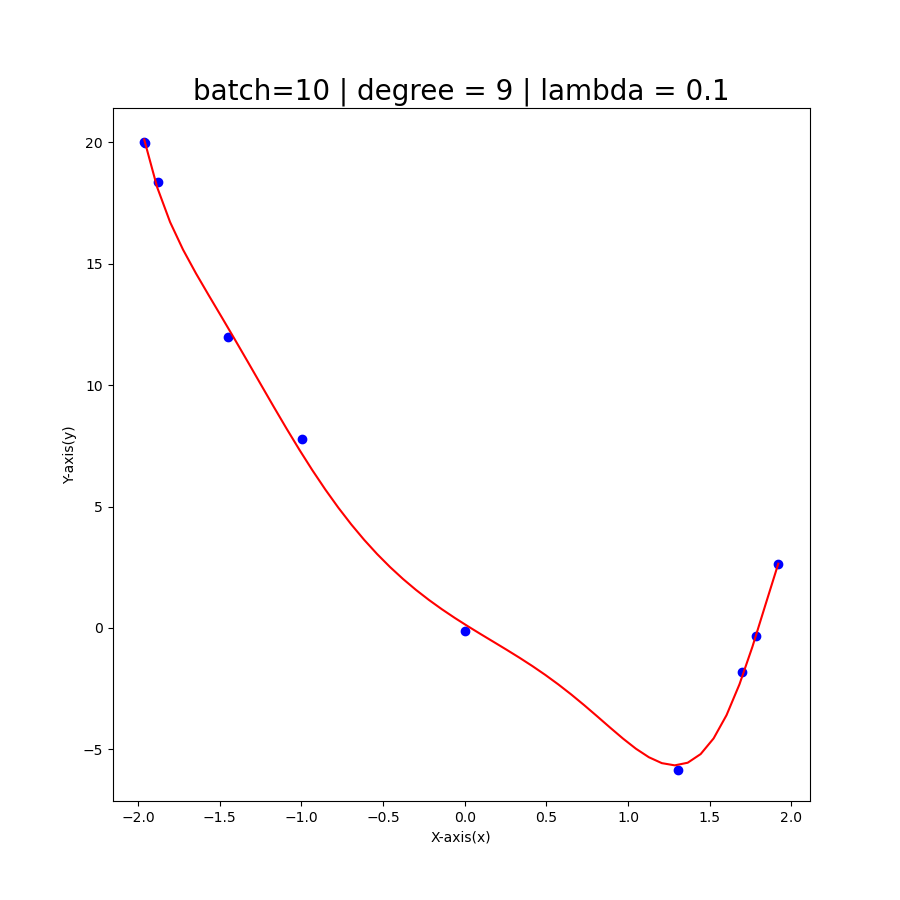
\includegraphics[height=2in]{Task 1 Images/Batch 10/Figure_7.png}
    \end{subfigure}%
    ~ 
    \begin{subfigure}[ht]{0.5\textwidth}
        \centering
        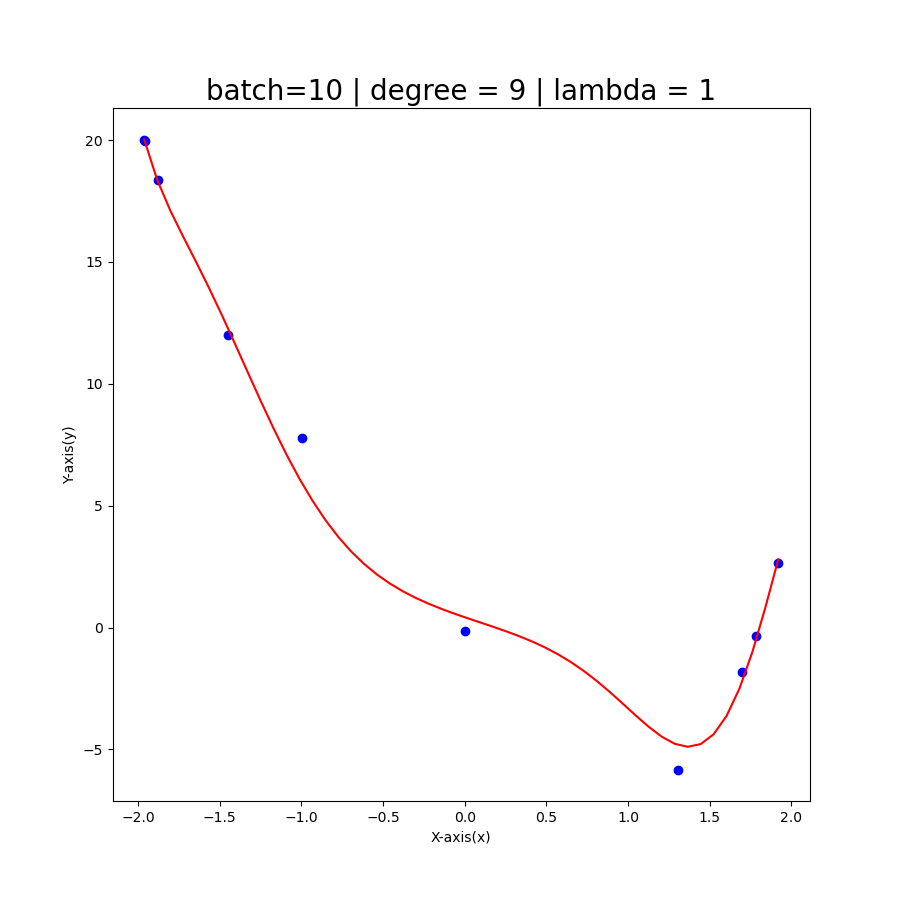
\includegraphics[height=2in]{Task 1 Images/Batch 10/Figure_8.png}
    \end{subfigure}%
    
\end{figure}

\begin{figure}[!ht]
    \centering
    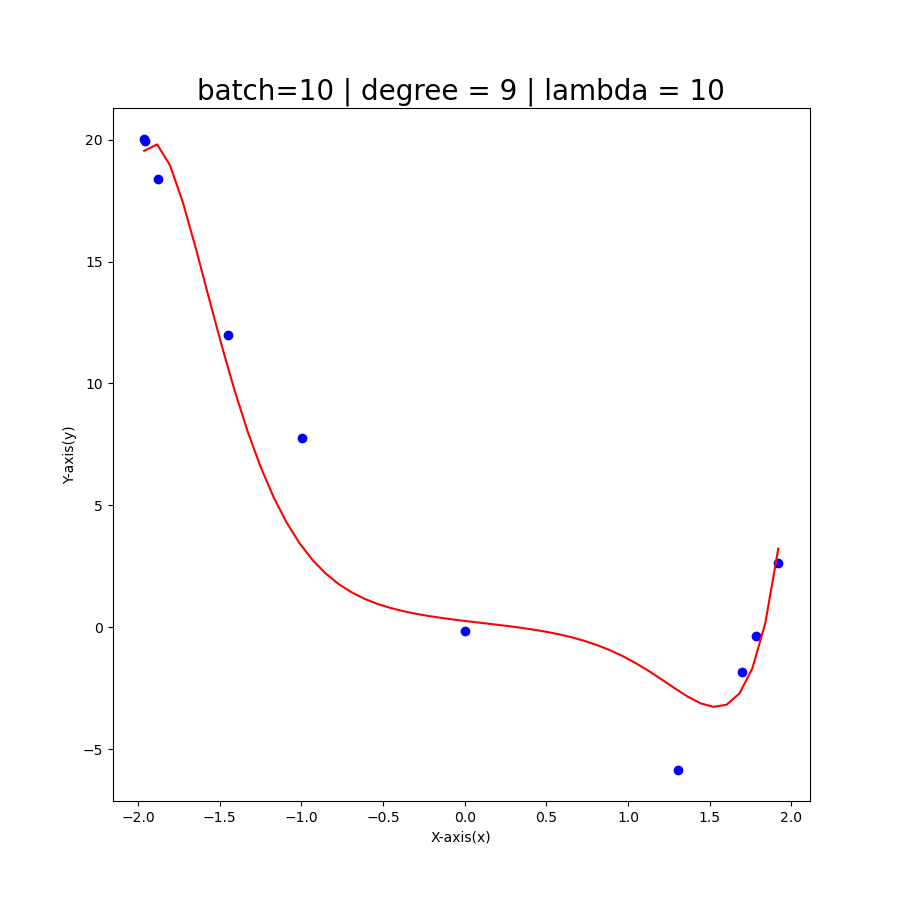
\includegraphics[height=2in]{Task 1 Images/Batch 10/Figure_9.png}
    \caption{Plots of degree 9 Polynomials having various orders of regularisation parameter using batch size=10}
    \label{fig:2}
\end{figure}

{\rowcolors{3}{green!40!yellow!10}{green!0!yellow!30}
\begin{table}[!ht]
\begin{tabular}{ |p{1.5cm}|p{3cm}|p{3cm}| p{3cm}|  }
\hline
\multicolumn{4}{|c|}{$\mathbf{E}_{rms}$ values for different regularisation parameters } \\
\hline
\rowcolor{lightgray} \textbf{lambda} & $\mathbf{E}_{rms-train}$ & $\mathbf{E}_{rms-test}$ & $\mathbf{E}_{rms-valid}$ \\
0.001   &   0.01  &  0.16   &  0.14   \\   
\hline
 0.01   &  0.05 &  0.09  &  0.21   \\   
 \hline
 0.1   &   0.28   &   0.20   &   0.45         \\
 \hline
 1   &   0.71   &    0.41        &     1.15     \\
 \hline
  10   &   1.91   &    0.64        &     2.57     \\
 \hline
\end{tabular}
\caption{Error comparisons for various regularisation parameters with degree=9 for Dataset 1 using batch size=10}
\label{table:2}
\end{table}
}


\subsection{Results for change in regularisation parameter and degree of fit for training data = 200}
Generally at lower degrees, the function does not well fit as can be observed from the plots [\ref{fig:3}]. The fit for degree 6 & 9 seems to be good. Since the validation accuracy is good and the model doesn't seem to overfit, regularisation experiment is not done here.


\begin{figure}[!ht]
    \centering
    \begin{subfigure}[t]{0.25\textwidth}
        \centering
        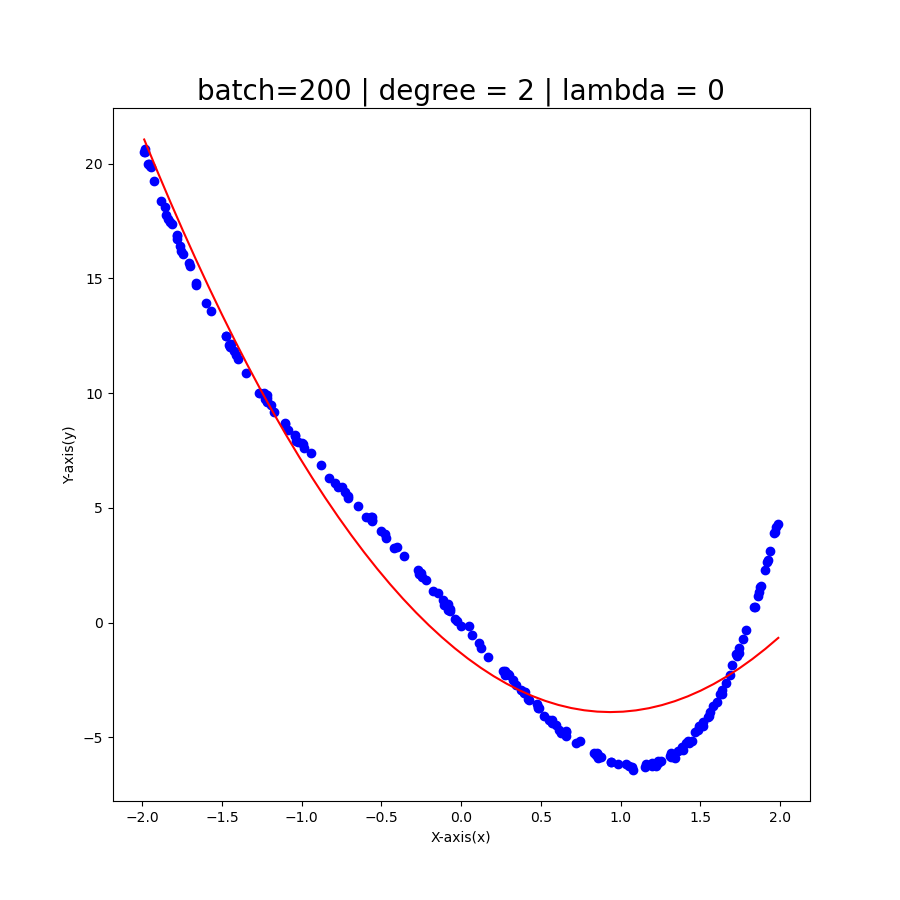
\includegraphics[height=1.5in]{Task 1 Images/Batch 200/Figure_1.png}
    \end{subfigure}%
    ~ 
    \begin{subfigure}[t]{0.25\textwidth}
        \centering
        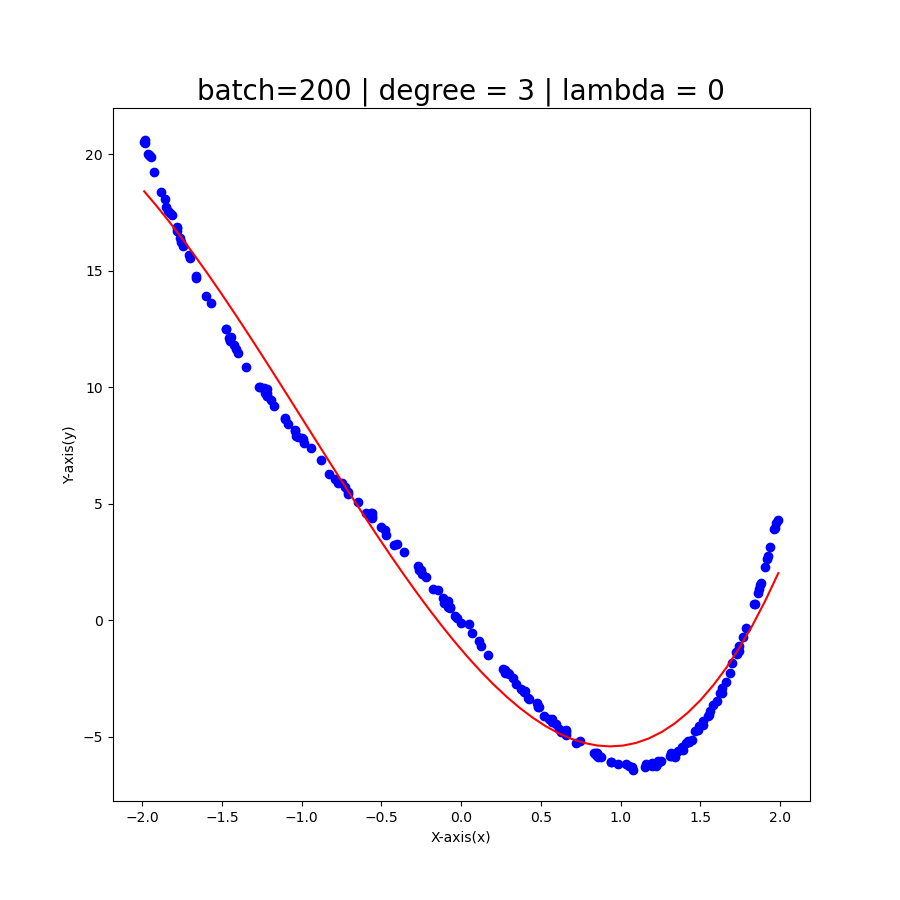
\includegraphics[height=1.5in]{Task 1 Images/Batch 200/Figure_2.png}
    \end{subfigure}%
    ~
    \begin{subfigure}[t]{0.25\textwidth}
        \centering
        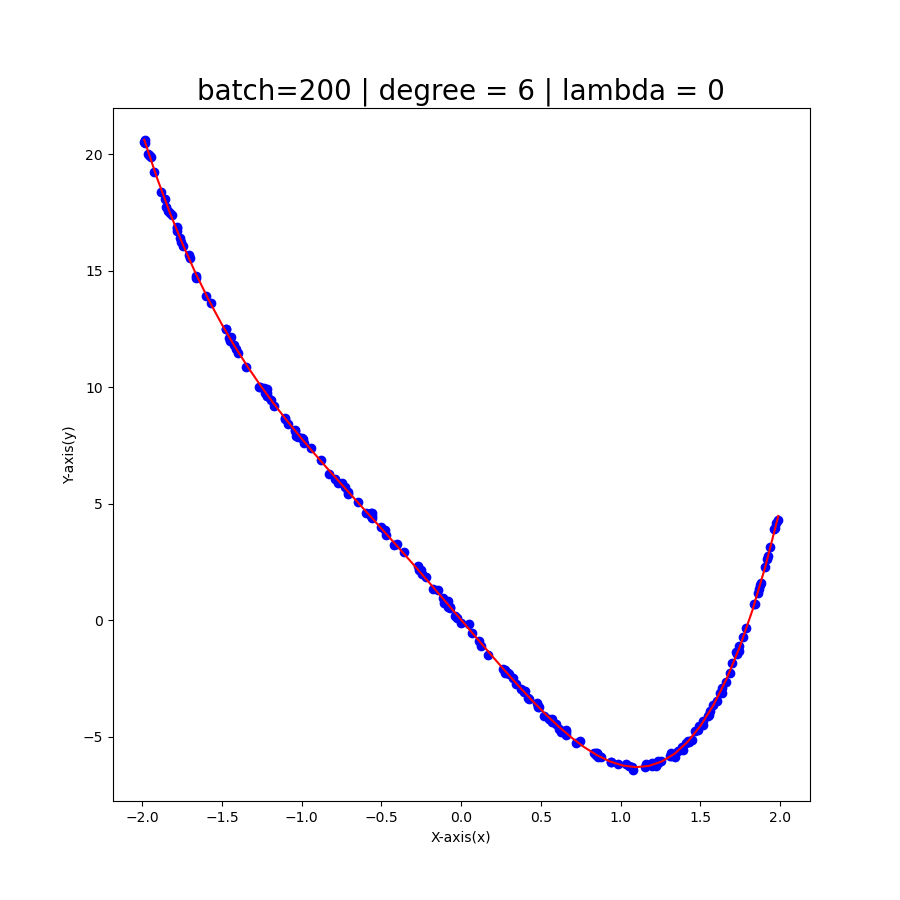
\includegraphics[height=1.5in]{Task 1 Images/Batch 200/Figure_3.png}
    \end{subfigure}%
    ~ 
    \begin{subfigure}[t]{0.25\textwidth}
        \centering
        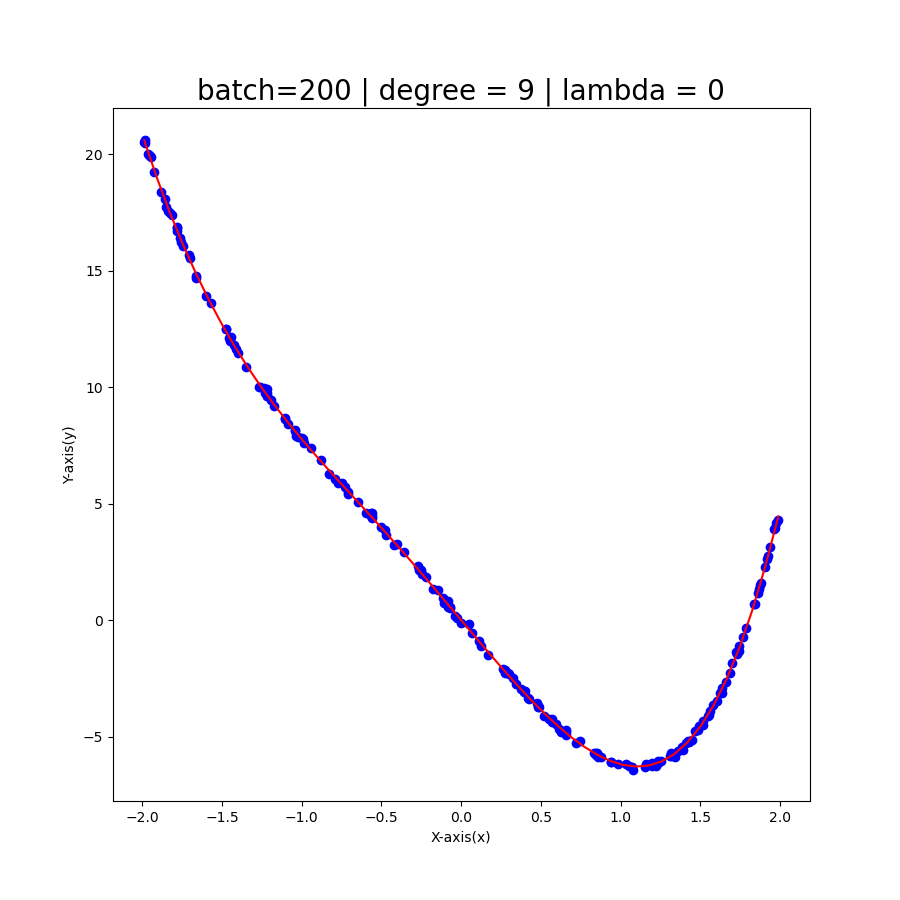
\includegraphics[height=1.5in]{Task 1 Images/Batch 200/Figure_4.png}
    \end{subfigure}%
    \caption{Plots of Polynomials having various orders of degree for a fixed regularisation parameter $\lambda = 0$ using batch size200}
    \label{fig:3}
\end{figure}




{\rowcolors{3}{green!40!yellow!10}{green!0!yellow!30}
\begin{table}[!ht]
\begin{tabular}{ |p{1.5cm}|p{3cm}|p{3cm}| p{3cm}|  }
\hline
\multicolumn{4}{|c|}{$\mathbf{E}_{rms}$ values for different degrees } \\
\hline
\rowcolor{lightgray} \textbf{Degree} & $\mathbf{E}_{rms-train}$ & $\mathbf{E}_{rms-test}$ & $\mathbf{E}_{rms-valid}$ \\
2   &   1.64  &  1.73   &  1.70   \\   
\hline
 3   &  1.05 &  0.85  &  1.07   \\   
 \hline
 6   &   0.09   &   0.09   &   0.11         \\
 \hline
 9   &  0.09   &    0.09        &     0.11     \\
 \hline
\end{tabular}
\caption{Error comparisons for varying degrees of $\phi(\mathbf{x}) $ for Dataset 1 using batch size=200}
\label{table:3}
\end{table}
}